\RequirePackage[l2tabu, orthodox]{nag}

%\documentclass[final, pdftex, a4paper, 12pt, openbib, ]{article}
\documentclass[final, a4paper, openbib, ]{article}
\usepackage[utf8]{inputenc}
\usepackage[french]{babel}
%\usepackage{fontspec}
%\usepackage{lmodern}
\usepackage[T1]{fontenc}
%\usepackage{graphicx}
\usepackage{alltt}
\usepackage{float}
%\usepackage{times}
%\usepackage{a4wide}
\usepackage{upquote,textcomp}
\usepackage{geometry}
%\usepackage{hyperref}
\usepackage{ulem}
\usepackage[
%pdftex,
final,                      % if you do    want to have clickable-colorful links
pdfstartview = FitV,
linktocpage  = false,       % ToC, LoF, LoT place hyperlink on page number, rather than entry text
breaklinks   = true,        % so long urls are correctly broken across lines
pagebackref  = false,     % add page number in bibliography and link to position in document where cited
]{hyperref}
\usepackage{mathtools}
\geometry{a4paper, portrait, margin=2cm}
%\addtolength{\textheight}{2 cm}
%\addtolength{\oddsidemargin}{-1cm}
%\addtolength{\topmargin}{-1cm}
%\addtolength{\textwidth}{1 cm}

%Good solution for monospaces
%\usepackage{pxfonts} % Or palatino or mathpazo, changes all fonts to something sans
%\usepackage{eulervm} % only changes math fonts, i checked
%\usepackage[ttdefault=true]{AnonymousPro} %Only changes tt fonts
% WHICH ONE TO CHOOSE?
%\usepackage{pslatex}
%\usepackage[ttdefault=true]{AnonymousPro} %Only changes tt fonts
% \usepackage[varg, cmintegrals, cmbraces, ]{newtxtext,newtxmath} % libertine, uprightGreek (U.S.) or slantedGreek (ISO), 
% \usepackage{tgtermes}
% \usepackage{txfonts}
% \usepackage{mathptmx}
% \usepackage[scaled=.90]{helvet}
% \usepackage{courier}
% \usepackage{textcomp}     % required for special glyphs
% \usepackage{bm}   


\usepackage{caption}
\captionsetup[figure]{labelformat=empty}% redefines the caption setup of the figures environment in the beamer class.

%Inconsoloata, a little too light.
%\usepackage{inconsolata}
%\renewcommand{\ttdefault}{Consolas}
%\usepackage{fontspec} %Doesn't work with pdflatex
%\setmonofont{Consolas}

%\renewcommand*\familydefault{\ttdefault} %% Only if the base font of the document is to be typewriter style
%\newcommand\Fontvi{\fontsize{6}{7.2}\selectfont}

%Make tabularx center cells vertically
%\def\tabularxcolumn#1{m{#1}}
%\renewcommand{\tabularxcolumn}[1]{>{\small}m{#1}}

%%Syntax hilighting
%\usepackage{fancyvrb}
\usepackage{minted}
%\usepackage[newfloat]{minted}
\usemintedstyle{borland}
%\usepackage{etoolbox}
%\AtBeginEnvironment{minted}{\singlespacing%
%	\fontsize{14}{14}\selectfont}
%\newminted{java}{fontsize=\footnotesize}
\usepackage{caption}

%\usepackage{multicol}
%\usepackage{vwcol}
%\usepackage{lipsum}
%\usepackage{microtype}
%\setlength{\columnseprule}{0.4pt}
%\renewcommand{\columnseprulecolor}{\color{red}}
\newcommand{\BAD}[1]{{\color{red}#1}}
\newcommand{\GOOD}[1]{{\color{darkgreen}#1}}


\usepackage{graphicx}
\usepackage{colortbl,array}
\usepackage{tabularx}
\definecolor{warningbackground}{RGB}{252,226,158}

\newcommand{\alertwarningbox}[1]{
	\centering
	\begin{tabularx}{0.9\linewidth}{
			>{\columncolor{warningbackground}}c
			>{\columncolor{warningbackground}}X}
		\raisebox{\dimexpr2\baselineskip-\height}
		{
\includegraphics[scale=0.8]{\images/Information.pdf}}&
		\raisebox{\tabcolsep}{\strut}#1\raisebox{-\tabcolsep}{\strut}
	\end{tabularx}
}


\usepackage{xcolor}

%\definecolor{infobackground}{RGB}{217,237,247}
%\definecolor{infoforeground}{RGB}{58,135,173}
%\definecolor{infoborder}{RGB}{188,232,241}

\definecolor{infobackground}{RGB}{217,237,247}
\definecolor{infofrancaisforeground}{RGB}{30,50,70}
\definecolor{infoborder}{RGB}{30,50,70}

\definecolor{infobackground}{RGB}{217,237,247}
\definecolor{infoforeground}{RGB}{30, 80, 150}
\definecolor{infoborder}{RGB}{47, 87, 232}

% ORANGE
\definecolor{infobackground2}{RGB}{255,210,180}
\definecolor{infoforeground2}{RGB}{212, 50, 0}
\definecolor{infoborder2}{RGB}{255, 90, 20}

% GREEN
\definecolor{infobackground3}{RGB}{223,251,223}
\definecolor{infoforeground3}{RGB}{25, 150, 25}
\definecolor{infoborder3}{RGB}{55, 220, 55}


\usepackage{environ}
\usepackage{tikz}
\usetikzlibrary{fit,backgrounds,calc}

\NewEnviron{alertinfo}[1]
{
	\begin{center}
		\begin{tikzpicture}
		\node[inner sep=0pt,
		draw=infoborder,
		line width=1pt,
		fill=infobackground] (box) {\parbox[t]{0.99\textwidth}
			{%
				\begin{minipage}{.12\textwidth}
				\centering\tikz[scale=3]
				\node[scale=1]
				{
					
\includegraphics[scale=0.25]{\images/Information.pdf}
				};
				\end{minipage}%
				\begin{minipage}{.86\textwidth}
				\vskip 10pt
				\textbf{\textcolor{infoforeground}{\large #1}}\par\smallskip
				\textcolor{infoforeground}{\large \BODY}
				\par\smallskip
				\par\smallskip
				\end{minipage}\hfill
			}%
		};
		\end{tikzpicture}
	\end{center}
}


\NewEnviron{alertinfo2}[1]
{
\begin{center}
    \begin{tikzpicture}
    \node[inner sep=0pt,
          draw=infoborder2,
          line width=1pt,
          fill=infobackground2] (box) {\parbox[t]{0.99\textwidth}
        {%
            \begin{minipage}{.12\textwidth}
                \centering\tikz[scale=3]
                \node[scale=1]
                {
                    
\includegraphics[scale=0.25]{\images/Information_orange.pdf}
                };
            \end{minipage}%
           \begin{minipage}{.86\textwidth}
                \vskip 10pt
                \textbf{\textcolor{infoforeground2}{\large #1}}\par\smallskip
                \textcolor{infoforeground2}{\large \BODY}
                \par\smallskip
                \par\smallskip
            \end{minipage}\hfill
        }%
    };
    \end{tikzpicture}
\end{center}
}

\NewEnviron{alertinfo3}[1]
{
\begin{center}
    \begin{tikzpicture}
    \node[inner sep=0pt,
          draw=infoborder3,
          line width=1pt,
          fill=infobackground3] (box) {\parbox[t]{0.99\textwidth}
        {%
            \begin{minipage}{.12\textwidth}
                \centering\tikz[scale=3]
                \node[scale=1]
                {
                    
\includegraphics[scale=0.25]{\images/Information_green.pdf}
                };
            \end{minipage}%
           \begin{minipage}{.86\textwidth}
                \vskip 10pt
                \textbf{\textcolor{infoforeground3}{\large #1}}\par\smallskip
                \textcolor{infoforeground3}{\large \BODY}
                \par\smallskip
                \par\smallskip
            \end{minipage}\hfill
        }%
    };
    \end{tikzpicture}
\end{center}
}

\usepackage{titling}

\newif\ifDRAFT
\DRAFTtrue
% Only comment and uncomment false line :
%\DRAFTfalse

\ifDRAFT
	%Hilighting commands:
	\newcommand{\hl}[1]{\textcolor{green}{#1}}
	\newcommand{\fix}[1]{\textcolor{red}{#1}}	
	\newcommand{\todo}[1]{{\color{red}\bf\em TODO:\/\@#1}}
%	\newcommand{\todo}[1]{{}}	
	\newcommand{\comment}[1]{{\color{blue}\bf\em Comment: \/\@#1}}
%	\newcommand{\comment}[1]{{}}	
	
	\newcommand{\hll}[1]{\textcolor{orange}{\sout{#1}}}
	%\newcommand{\hll}[1]{{}}
	\newcommand{\WR}[1]{\textcolor{purple}{#1}}
\else
	% for final sub
	\newcommand{\hl}[1]{#1}	
	%\newcommand{\hl}[1]{\textcolor{dkgreen}{#1}}
	\newcommand{\fix}[1]{{}}
%	\newcommand{\fix}[1]{\textcolor{red}{#1}}
	\newcommand{\todo}[1]{{}}
	\newcommand{\hll}[1]{{}}
	\newcommand{\comment}[1]{{}}
	\newcommand{\WR}[1]{{#1}}
%	\newcommand{\WR}[1]{\textcolor{purple}{#1}}	
\fi


\newcommand{\codes}{codes}
\newcommand{\images}{images}

%FIX FOR : Undefined control sequence. \tightlist
\providecommand{\tightlist}{%
  \setlength{\itemsep}{0pt}\setlength{\parskip}{0pt}}
  
%\title{GBIAAL 4$^{\mbox{\`eme}}$ année \\ Devoir Surveillé --- Base de données \\ 13 janvier 2016  \\ 1 heure}
%\title{GIS 3$^{\mbox{\`eme}}$ année
	%\\TP1 Structures, Listes contiguës, Redirections}
%}
%\author{\huge \textbf{Introduction à} \\  \Huge\textbf{\texttt{git}}}
\setlength{\parindent}{0pt}
%\pagestyle{empty}
\title{Spécialités GIS / IMA 3$^{\mbox{\`eme}}$ année\\
\huge \textbf{Introduction outil \texttt{GIT}
}}
\setlength{\parindent}{0pt}
%\pagestyle{empty}
\author{\copyright{} W. Rudametkin -- Polytech Lille\\
	Adaptation~: M.E. Kessaci, O. Caron, J. Dequidt}
\date{\Large \url{https://rudametw.github.io/teaching/}}% \\ Polytech Lille}

%\author{Walter Rudametkin}
%\institute[Polytech Lille]{
%Walter.Rudametkin@polytech-lille.fr\\
%\url{https://rudametw.github.io/teaching/}\\
%\vspace{0.5cm}Bureau F011\\
%Polytech Lille\\

\begin{document}
%\vspace{-15cm}
\vspace{-5cm}
\posttitle{\par\end{center}}
\setlength{\droptitle}{-45pt}
\maketitle
%\thispagestyle{empty}

\vspace{-1.2cm}
\section{Objectifs}\label{objectifs}

\begin{itemize}
\item Apprendre à se servir d'un Logiciel de Gestion de Versions\footnote{\url{https://fr.wikipedia.org/wiki/Logiciel_de_gestion_de_versions}}.
\item Maîtrisez le versionnement d'un projet logiciel.
\item Partager un projet et travailler en équipe.
\end{itemize}

\begin{alertinfo}{IMPORTANT !}
Lisez attentivement la sortie de \textbf{\textit{chaque}} commande \texttt{git}.
Il est fortement conseillé de travailler exclusivement sur terminal pour ce TP.
\end{alertinfo}

\section{Contexte et préparation}
\label{context} 

\subsection{Configuration de votre environnement}

\paragraph{\texttt{.bashrc} et \texttt{git-prompt.sh}}
Nous vous fournissons une configuration avancée de \texttt{bash} (l'interpréteur en ligne de commande utilisé par défaut) avec une aide GIT intégré.
Utiliser un prompt spécial GIT est très pratique pour visualiser rapidement où vous en êtes (connaître la branche sur laquelle vous travaillez par exemple). La commande suivante exécute un script shell qui modifie votre prompt, nous vous proposons une qui est simple, git-prompt.sh\footnote{\url{https://github.com/git/git/blob/master/contrib/completion/git-prompt.sh}}. Ce prompt ne sera actif que dans les répertoires de vos projets GIT~: 
\begin{minted}[mathescape=true,escapeinside=||,tabsize=4
%	,fontsize=\footnotesize,
]{bash}
	source ~wrudamet/public/bashrc-students
\end{minted}
%source ~ocaron/public/git/config_git

Pour ne pas devoir lancer cette commande à chaque connexion, vous pouvez l'insérer au début de votre fichier \texttt{\~{}/.bashrc}.

\begin{alertinfo3}{Astuce si vous êtes sur votre ordinateur personnel !}
Optionnellement, à l'aide de \texttt{scp}, \texttt{rsync} ou un outil graphique qui supporte le protocole \texttt{sftp}, vous pouvez copier le fichier \mintinline{bash}{~wrudamet/public/bashrc-students} pour adapter votre \mintinline{bash}{fichier ~/.bashrc} local et télécharger \mintinline{bash}{git-prompt.sh}, en suivant la documentation, pour intégrer le support de git manuellement.
\end{alertinfo3}

%\begin{minted}[mathescape=true,escapeinside=||,tabsize=4
%%	,fontsize=\footnotesize,
%]{bash}
%	~wrudamet/public/set_bashrc.sh
%\end{minted}
%
%Pour les curieux, vous pouvez regarder vos fichiers \mintinline{bash}{~/.bashrc}, \mintinline{bash}{~/.bashrc-students} et \mintinline{bash}{~/git-prompt.sh} pour comprendre ce qui a été ajouté.
%N'hésitez pas à éditer ou supprimer les changements si vous préférez.

\paragraph{Terminaux}
%\WR{Copier le fichier XXX.aide pour récupèrer quelques commandes. }
Nous vous proposons de travailler sur plusieurs terminaux ouverts simultanément, une disposition possible est indiquée dans la figure~\ref{terminals} mais vous pouvez les ranger à votre convenance tout au long du TP.
\begin{figure}[h]
	\centering
	{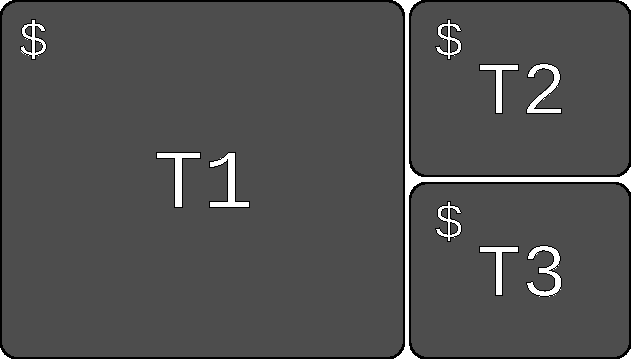
\includegraphics[scale=0.45]{images/terminals.pdf}}
	\caption{Figure 1: Disposition proposée des terminaux}
	\label{terminals}
\end{figure}

Cette disposition vous permettra d'exécuter vos commandes \texttt{git} dans le terminal \texttt{T1}, tout en exécutant des commandes de \textit{suivi} dans les terminaux \texttt{T2} et \texttt{T3}.
Dans un premier temps, positionnez \texttt{T1}, \texttt{T2} et \texttt{T3} dans le répertoire où vous allez travailler via la commande \texttt{cd}.\\

La commande \texttt{watch}\footnote{\url{https://en.wikipedia.org/wiki/Watch\_(Unix)}} permet de répéter une commande toute les $X$ secondes et la commande \texttt{tree} permet de visualiser toute l'arborescence de dossiers fichiers. Dans le terminal \texttt{T2} nous allons surveiller le répertoire \texttt{tpgit}, alors exécutez :
\begin{minted}[mathescape=true,escapeinside=||,tabsize=4
%	,fontsize=\footnotesize,
]{bash}
	watch -d -n3 tree -a tpgit
\end{minted}

Et dans le terminal \texttt{T3} exécutez :
\begin{minted}[mathescape=true,escapeinside=||,tabsize=4
%	,fontsize=\footnotesize,
]{bash}
	watch cat ~/.gitconfig
\end{minted}

Il est normal que ces commandes affichent pour le moment des erreurs car nous n'avons pas encore créé le répertoire \texttt{tpgit} ni le fichier \texttt{.gitconfig}. N'hésitez pas à réduire la taille de police des terminaux pour mieux afficher les informations plus tard, la sortie des commandes va grandir rapidement.


\subsection{Configuration de votre compte \texttt{git}}

Dans un projet géré par plusieurs, il est important de savoir qui a fait quoi. \texttt{git} a donc besoin d'une configuration pour identifier vos futurs \textit{commits}, et vous pouvez également spécifier certains comportements.
Les commandes suivantes vont modifier votre fichier \texttt{.gitconfig}, tapez les une à une en regardant les changements dans le terminal \texttt{T3}:

\begin{minted}[mathescape=true,escapeinside=||,tabsize=4
%	,fontsize=\footnotesize,
]{bash}
	git config |-{}-|global user.name "votre nom"
	git config |-{}-|global user.email nom.prenom@polytech-lille.net
	git config |-{}-|global push.default simple
	git config |-{}-|global color.decorate full
	git config |-{}-|global merge.conflictstyle diff3
	git config |-{}-|global core.editor 'nano'
\end{minted}

Si vous préférez un autre éditeur à la place de \texttt{nano}, vous pouvez l'utiliser (\textit{e.g.,} \texttt{kate -b}, \texttt{vim}, \texttt{emacs}, \texttt{gedit}).

\begin{alertinfo}{Rappel !}
Les configurations de \texttt{git} et de \texttt{bash} doivent se faire une fois pour chaque compte.
Votre binôme devra réaliser la même configuration sur son compte, et si vous comptez travailler sur un autre PC, il faudra récupérer votre fichier \texttt{.gitconfig} ou relancer les commandes de configuration.
\end{alertinfo}

\section{Initialisation d'un dépôt \texttt{git}}

Nous allons travailler sur un projet qu'on appellera \texttt{tpgit}.
En vous aidant des supports du cours (\textit{e.g.,} slide 12), vous devez~:
\begin{itemize}
\item créer un répertoire \texttt{tpgit}
\item initialiser dans ce répertoire un dépôt git vide
\item regarder les fichiers créés pour ce dépôt, ils seront affichés dans le terminal \texttt{T2} dans le dossier \texttt{.git}
\item créer un fichier \texttt{fruits.txt}
\item réaliser un commit en ajoutant 2 fruits à \texttt{fruits.txt}.
Pour rappel, l'enchaînement des commandes est : \mintinline{bash}{status, add, status, commit, status, log}.
\textbf{Lisez la sortie de chaque commande} pour comprendre leur fonctionnement.
\item réaliser 3 commits de plus en ajoutant à chaque fois des fruits.
\end{itemize}

\begin{alertinfo3}{Astuce !}
Utilisez les commandes \texttt{git status}, \texttt{git diff \textit{nom\_fichier}} et \texttt{git log} pour comprendre l'état de votre dépôt. La commande \texttt{git log -}\texttt{-graph -}\texttt{-oneline -}\texttt{-decorate -}\texttt{-all} vous donne une historique détaillé et globale avec toutes les branches, étiquettes et commits.
\end{alertinfo3}

Dans le terminal \texttt{T3}, arrêter le processus (\texttt{ctrl+c}) et exécuter la commande suivante dans le répertoire \texttt{tpgit} pour visualiser l'historique du dépôt~: \verb+watch git log --graph --oneline --decorate --all+ . Si vous voulez avoir une sortie colorée, vous pouvez ajouter l'option \verb+--color+ aux commandes \texttt{watch} et \texttt{git} comme suit : \verb+watch --color git log --graph --oneline --decorate --all --color+

\section{Branches \texttt{git}}

Branches \texttt{legumes}
\begin{itemize}
\item créer une branche \texttt{legumes}, se placer dans cette branche (vérifier avec le prompt ou avec la commande \texttt{git branch} que vous êtes bien sur la branche \texttt{legumes})
\item ajouter un fichier \texttt{legumes.txt} sur cette branche
\item réaliser 3 commits différents en ajoutant des légumes à \texttt{legumes.txt}
\item vérifier l'historique de vos commits à l'aide de \texttt{git log}.
\end{itemize}

Branches \texttt{sauces}
\begin{itemize}
\item créer une branche \texttt{sauces}
\item ajouter un fichier \texttt{sauces.txt} sur cette branche
\item réaliser 2 commits différents
\item vérifier l'historique de vos commits et l'existence de \textbf{3 branches} (master, legumes, sauces) à l'aide de \texttt{git branch} et \texttt{git log}.
\end{itemize}


\section{Merges \texttt{git}}
Vous avez décidé que vos commits dans les branches \texttt{legumes} et \texttt{sauces} sont pertinents, maintenant vous devez les intégrer dans \texttt{master}.
\begin{itemize}
\item aller sur la branche \texttt{legumes}
\item vérifier l'état de votre espace de travail (\textit{e.g.,} l'inexistence du fichier \texttt{sauces.txt})
\item merger \texttt{master} dans \texttt{legumes}
\item si tout c'est bien passé, merger \texttt{legumes} dans \texttt{master}
\item vérifier l'historique de vos commits et l'apparition de \texttt{legumes.txt} sur la branche \texttt{master}\\
\end{itemize}

Vous pouvez maintenant merger la branche \texttt{sauces} avec \texttt{master} en suivant le même processus.
Vérifiez que tous les branches sont à jour.

\section{Dépôt distant}

%%%Gitlab.com
%Nous allons créer vos comptes sur le serveur GitLab de \url{https://gitlab.com}.
%Connecter-vous sur \url{https://gitlab.com/users/sign_in} et créer votre compte en utilisant votre email de Polytech\footnote{Pour information, vous pouvez également activer votre compte sur le serveur gitlab de l'Université de Lille \url{https://gitlab.univ-lille.fr} ou le serveur gitlab de Polytech \url{https://archives.plil.fr}.}.
%Nous vous recommandons d'utiliser votre login Polytech comme \texttt{username} pour faciliter les opérations de \texttt{push} et \texttt{pull} plus tard.

Nous allons activer vos comptes sur le serveur GitLab de l'Université de Lille (\url{https://gitlab.univ-lille.fr}) et créer un dépôt vide où vous allez pousser votre dépôt existant \texttt{tpgit}. (Vous êtes également libre d'utiliser Github, GitLab.com, ou le serveur GitLab de Polytech \url{https://archives.plil.fr/}.)

GitLab vous permet de gérer votre projet et fourni plusieurs fonctionnalités intéressantes (\textit{e.g.,} issues, graphes, édition de fichiers, recherche de contributeurs, dashboard).\\


%Vous allez devoir (procédure plus précise décrite après):
%\begin{itemize}
%\item se connecter sur \url{https://gitlab.univ-lille.fr}
%%\item se connecter sur \url{https://gitlab.com}
%\item créer un projet sur le GitLab (NE PAS COCHER \textit{INITIALIZE REPOSITORY !})
%\item pousser votre dépôt \texttt{tpgit} sur le GitLab
%\item ajouter votre binôme aux membres de votre projet avec, au minimum, le niveau de droit \textit{Developer} (il devra créer son compte et se connecter une première fois avant d'apparaître dans la liste des membres)
%\end{itemize}

%Vous allez devoir (procédure plus précise décrite après):
%\begin{itemize}
%\item se connecter sur \url{https://gitlab.univ-lille.fr}
%%\item se connecter sur \url{https://gitlab.com}
%\item créer un projet sur le GitLab (NE PAS COCHER \textit{INITIALIZE REPOSITORY !})
%\item pousser votre dépôt \texttt{tpgit} sur le GitLab
%\item ajouter votre binôme aux membres de votre projet avec, au minimum, le niveau de droit \textit{Developer} (il devra créer son compte et se connecter une première fois avant d'apparaître dans la liste des membres)
%\end{itemize}

\begin{alertinfo2}{Attention !}
Il y a deux protocoles réseau pour échanger avec GitLab, HTTPS et SSH. Nous vous conseillons de travailler avec HTTPS dans un premier temps.
Dans le futur vous pouvez choisir SSH, qui est plus puissant et flexible, mais il faudra configurer vos clés privés et publiques en suivant l'aide \url{https://gitlab.com/help/ssh/README\#generating-a-new-ssh-key-pair}
\end{alertinfo2}
%\url{https://gitlab.univ-lille.fr/help/ssh/README} ou \url{https://archives.plil.fr/help/ssh/README}


\paragraph{Créer un dépôt sur GitLab et poussez \texttt{tpgit}}
\begin{enumerate}
\item Se connecter sur \url{https://gitlab.univ-lille.fr}
\item Cliquer sur \textit{New Projet} en haut pour créer un nouveau projet
\item Donner un nom à votre projet et cliquer sur \textit{Create project} (\underline{NE PAS COCHER \textit{Initialize Repository !}})
\item Vous êtes emmenés dans votre projet, qui est vide, avec les instructions des différentes formes d'initialisation.
\textbf{Lisez les propositions.}
Vous devez \textbf{impérativement vérifier et changer l'url de \texttt{SSH} à \texttt{HTTPS}} si vous n'avez pas configuré des clés SSH pour vos connexions.
\item Retrouvez les instructions \textit{Push an existing Git repository}. Vous allez copier et exécuter la commande :\\ \texttt{git remote add origin https://gitlab.com/<user>/<project.git>} avec le bon url suivi de\\ \texttt{git remote -v} pour vérifier le dépôt, et \texttt{git push -u origin master} pour indiquer que vous voulez envoyer la branche actuelle vers la branche \texttt{master} du dépôt distant surnommé \texttt{origin}.
\item Rafraîchissez la page de votre projet GitLab, votre projet \texttt{tpgit} doit s'y retrouver.
\item Naviguez votre projet sur Gitlab pour voir l'historique de commits, vos fichiers, vos graphes, etc.
\end{enumerate}	

\paragraph{Gestion des membres de votre projet.}
Ajouter votre binôme aux membres de votre projet avec, au minimum, le niveau de droit \textit{Developer} (il devra créer son compte et se connecter une première fois avant d'apparaître dans la liste des membres)
\begin{enumerate}
\item Aller dans les \textit{Settings} de votre projet (menu de gauche),
\item Cliquer sur \textit{Members} dans le menu \textit{Settings} (menu de gauche),
\item Cliquer sur \textit{New project member} en haut à droite,
\item Chercher le login de la personne que vous voulez ajouter (votre binôme),
\item Sélectionner le niveau de droit de cette personne (\textit{Developer}),
\item Cliquer sur \textit{Add users}.
\item Cliquer sur \textit{Protected branches} dans le menu \textit{Settings} (menu de gauche), \textit{Repository},
%puis cliquer la case à cocher \textit{Developers can push} pour la branche "master" du projet (bas de l'écran principal).
puis cliquer sur \textit{Protected branches} et cliquer sur \textit{Unprotect} pour la branche \texttt{master}
\end{enumerate}


\section{Travail collaboratif}


Vous allez travailler en binôme sur le dépôt de binôme 1. 
Binôme 2 doit donc cloner le projet de binôme 1 dans un dossier nommé tg-git-binôme.
Pour cela :
\begin{itemize}
\item Binôme 2 doit se connecter sur le projet de binôme 1 dans GitLab %\url{https://archives.plil.fr/<login>/<projet.git>}
\item Cliquer sur HTTPS
\item Cloner le projet à l'aide de la commande \texttt{git clone <url> tp-git-binome}
\item Regardez l'historique du projet.
\end{itemize}

\section{Travail simultané}

Vous allez travailler en même temps sur ce projet commun, chacun sur son propre dépôt local (binôme 1 sur son dossier local originel, et binôme 2 sur son nouveau dossier local tp-git-binome), et vous allez synchroniser les changements après.

\subsection{Merge sans conflit}

\paragraph{Travail de Binôme1}
\begin{itemize}
\item créer une branche \texttt{epices}
\item ajouter un fichier \texttt{epices.txt} sur cette branche
\item réaliser 2 commits différents
\item merger vos commits dans \texttt{master}
\item récupérer les changements sur le serveur (\texttt{git pull})
\item pousser vos changements vers le serveur GitLab à l'aide de la commande \texttt{git push}
\end{itemize}

\paragraph{Travail de Binôme2}
\begin{itemize}
\item créer une branche \texttt{herbes}
\item ajouter un fichier \texttt{herbes.txt} sur cette branche
\item réaliser 2 commits différents
\item merger votre branche dans \texttt{master}
\item récupérer les changements sur le serveur (\texttt{git pull})
\item pousser vos changements vers le serveur GitLab à l'aide de la commande \texttt{git push}\\
\end{itemize}

\paragraph{Tous les deux}
\begin{itemize}
\item vérifier l'existence des fichiers \texttt{epices.txt} et \texttt{herbes.txt} dans vos deux dépôts
\item vérifier l'historique des deux dépôts... est-ce que tous les ID de commits sont les mêmes ? Vous avez trouvé le dernier commit de merge ? Vous voyez les commits de votre binôme ?\\
\end{itemize}

Un de vous deux a été le premier à pousser, et l'autre a dû fusionner les changements avant de pouvoir pousser son travail.
Parce que vous avez travaillé sur des fichiers différents, le \texttt{merge} a été résolu automatiquement.
Nous allons maintenant vous obliger à générer des conflits et à les résoudre.

\begin{alertinfo3}{Astuce !}
Vous en avez marre de taper votre login et mot de passe à chaque \texttt{pull} et \texttt{push} ?
Git peut se souvenir de votre identité pendant un temps déterminé, par exemple, pour une heure utilisez la commande :\\
\texttt{git config \texttt{-}{}-global credential.helper 'cache \texttt{-}{}-timeout=3600'}
\end{alertinfo3}


\subsection{Merge avec conflit}

\paragraph{Générer un conflit}
\begin{itemize}
\item éditez tous les deux, chacun sur son dépôt, le fichier \texttt{fruits.txt}, de façon à \textbf{effacer} certains fruits et à \textbf{ajouter} des nouveaux (faites des changements différents)
\item commitez vos changements mais ne poussez pas encore
\item binôme1 pousse ses changements en premier
\item binôme2 pull les changements de binôme1 et\ldots CONFLIT !
\item \texttt{git status}, lisez la sortie
\item à l'aide du cours (slides 26-29), essayez de résoudre ce conflit
\item une fois résolu, fusionnez vos changements et poussez vers le serveur
\item binome1, récupérez les changements et vérifiez l'état de \texttt{fruits.txt}
\end{itemize}

\paragraph{Générer un 2ème conflit, inverser les rôles}
\begin{itemize}
\item comme précédemment, générer un conflit dans le fichier \texttt{legumes.txt} mais cette fois inversez les rôles :  binome2 pousse en premier, binome1 résout le conflit.
\item au moment du conflit, c'est-à-dire, tout de suite après un \texttt{git pull} ou \texttt{git merge}, vous pouvez annuler le merge avec la commande \texttt{git merge \texttt{-}{}-abort}.
Essayez la commande et vérifier que votre dépôt revient dans l'état avant le \texttt{pull} (plus de conflits, vérifier avec \texttt{status}).
Refaite \texttt{git pull} et vous allez retrouver le conflit, résolvez-le cette fois.
\end{itemize}

\begin{alertinfo3}{Astuce !}
Pour minimiser les conflits, il faut s'assurer que tout le monde maintienne son dépôt à jour.
Il faut régulièrement merger vers la branche \texttt{master}, faire \texttt{git pull} sur vos branches, et corriger les éventuels petits conflits quand ils sont simples.
Avant de pousser vos changements avec \texttt{git push}, il faut toujours faire un \texttt{git pull}.
\end{alertinfo3}

\section{Documenter votre projet à l'aide de Markdown}

Markdown est un langage de balisage léger, plus rapide à écrire que HTML et très flexible.
Il est interprété automatiquement par GitLab (et plein d'autres produits) et permet de documenter votre projet ou même d'écrire vos rapports.\\

Créez un fichier \texttt{README.md} à la racine de votre dépôt en utilisant la syntaxe markdown pour spécifier des titres, listes, des extraits de code.
Vous devez au minimum :
%\begin{itemize}
	\begin{itemize}
	\item donnez une description de votre projet
	\item listez les auteurs dans une section \textit{Auteurs}
	\item listez les objectifs dans une section \textit{Objectifs}\\
	\end{itemize}
%\end{itemize}

Vous pouvez vous inspirer de cet exemple sur Github :\\
\url{https://gist.github.com/PurpleBooth/109311bb0361f32d87a2}\\
(cliquer sur RAW pour avoir les sources).
Vérifiez que votre README s'affiche correctement sur GitLab.
%\url{https://gist.githubusercontent.com/PurpleBooth/109311bb0361f32d87a2/raw/824da51d0763e6855c338cc8107b2ff890e7dd43/README-Template.md}



\section{Eclipse et GIT (Optionnel)}

Sous Eclipse, il existe une extension GIT qui présente quelques avantages. La première est de développer et gérer les versions sans quitter Eclipse. La seconde permet de s'abstraire de la syntaxe des commandes en ligne. Des outils graphiques viennent également simplifier la gestion des conflits.

Voici un rapide tutoriel sur quelques commandes de base de cette extension.
\begin{enumerate}
	\item Sous Eclipse (\texttt{/usr/local/eclipseNeon/eclipse \&}, créer un projet PHP de nom \texttt{"demoPHP"}.
	\item {\bf Réalisez l'équivalent de \texttt{"git init"}}~:\\
	Sélectionnez le projet et, avec le clic droit de la souris, sélectionnez "Team/Share Project\ldots", sélectionnez "Git" puis cliquez sur \texttt{"Next>"}, cliquez sur "Create\ldots" (en haut à droite), sélectionnez un répertoire de nom "git\_demoPHP", cliquez sur \texttt{"Finish"}, cochez le projet \texttt{"demoPHP"} puis cliquez sur \texttt{"Finish"}.
	\item Créez un fichier \texttt{index.html} dans votre projet.
	\item {\bf Réalisez l'équivalent de \texttt{"git add ... ; git commit"}}~:\\
	Sélectionnez le projet et, avec le clic droit de la souris, sélectionnez "Team/Commit...". Une vue "Git Staging" est alors disponible. Déplacez le fichier \texttt{index.html} de la sous-fenêtre "Unstaged Changes" vers la sous-fenêtre "Staged Changes" (équivalent de \texttt{git add}), donnez un titre à votre futur commit dans la sous-fenêtre "Commit Message" puis cliquez sur "Commit" (équivalent de \texttt{git commit}).
	\item Connectez-vous sur \url{https://gitlab.univ-lille.fr} et créez un projet \texttt{"demoPHP"}, mémorisez l'adresse du projet~: \url{https://gitlab.univ-lille.fr/<votre_login>/demoPHP.git}
	\item {\bf Réalisez l'équivalent de \texttt{"git add ... ; git commit ; git push"}}~:\\
	c'est la même procédure que le point 4 mais il faut cliquer sur "Commit and Push" à la fin. Pour ce premier "push", une fenêtre de dialogue vous demande l'URI, saisissez \url{https://gitlab.univ-lille.fr/<votre_login>/demoPHP.git}, cliquez sur \texttt{"Next>"}, saisissez vos login/password puis cliquez sur \texttt{"OK"} et \texttt{"Finish"}.
	\item {\bf Réalisez l'équivalent de \texttt{"git pull"}}~:\\
	Il suffit de sélectionnez "Team/Pull" et suivre les instructions.
\end{enumerate}

A partir du menu "Team", vous disposez de l'équivalent de toutes les commandes \texttt{git}.

Pour créez un projet Eclipse à partir d'un projet déjà stocké dans le repository local ou distant, il faut sélectionnez dans le menu Eclipse "File/Import.../Git/Projects from Git" et suivre les inscriptions.

%Pour comprendre comment fonctionne l'extension \texttt{EGit} d'Eclipse, suivez ce tutoriel~:\\ \url{https://openclassrooms.com/courses/egit-quand-git-s-invite-dans-eclipse}
%
%{\bf Attention~:} vous devez passer la partie d'installation de \texttt{EGit}, cette extension est déjà installée.

\section{Continuer à apprendre}

Si vous voulez maîtriser \texttt{git}, n'hésitez pas à faire le tutoriel donné par le laboratoire CRIStAL de l'université de Lille.
Il y a beaucoup de fonctionnalités avancées qui peuvent s'avérer très utiles.
\url{http://www.cristal.univ-lille.fr/TPGIT/} .\\

Vous pouvez également consulter les liens suivants :
\paragraph{Liens, aides et outils}
\begin{itemize}
	\item Où stocker vos projets
	\begin{itemize}
		\item \url{https://gitlab.univ-lille.fr/}	
		\item \url{https://archives.plil.fr/}
		\item \url{https://about.gitlab.com/}
		\item \url{https://github.com/}
		\item \url{https://bitbucket.org/}
		\item Votre serveur perso (\textit{e.g.,} installer GitLab chez vous)
	\end{itemize}
	\item Tutoriels
	\begin{itemize}
		\item \url{http://www.cristal.univ-lille.fr/TPGIT/}
		\item \url{https://crypto.stanford.edu/~blynn/gitmagic/intl/fr/book.pdf}
		\item \url{https://learngitbranching.js.org/}
		\item \url{https://try.github.io/}
		\item \url{https://git-scm.com/book/fr/v2}
	\end{itemize}
	\item Vidéos
	\begin{itemize}
		\item \url{https://www.youtube.com/watch?v=OqmSzXDrJBk}
		\item \url{https://www.youtube.com/watch?v=uR6G2v_WsRA}
		\item \url{https://www.youtube.com/watch?v=3a2x1iJFJWc}
		\item \url{https://www.youtube.com/watch?v=1ffBJ4sVUb4}
		\item \url{https://www.youtube.com/watch?v=duqBHik7nRo}
	\end{itemize}
\end{itemize}
\end{document}
